\refstepcounter{section}
\section*{Lecture 28: Radiation dominated Universe}
\addcontentsline{toc}{section}{Lecture 28: Radiation dominated Universe}
In the previous section we saw scalar fields in the FLRW metric. Here we will focus on a period in the Universe's past when it was (perhaps) dominated by radiation (photns). For that, note that in Minkowski space, the electromagnetic action is given by  
\begin{align*}
    \Ss\tund{EM} = \int \dd^4 x \qty[-\frac{1}{4}F_{\mu\nu}F^{\mu\nu}]
\end{align*}
where $F_{\mu\nu}$ is Maxwell's field tensor as defined in Eq.\ref{eqn:fmunu}. Note that this action is Lorentz invariant and also enjoys gauge symmetry. To generalise this, we use our previous prescription, that is, we replace the measure with the invariant volume, introduce the general metric and change the partial derivatives to covariant derivatives, doing which we obtain the action in arbitrary curved spacetime
\begin{align}\label{eqn:elecaction}
    \Ss\tund{EM} = \int \dd^4 x \ \detm\  \qty[-\frac{1}{4}g^{\mu\alpha}g^{\nu \beta}F_{\mu\nu}F_{\alpha\beta}]
\end{align}
where $F_{\mu\nu} = \covd{\mu}A_\nu - \covd{\nu}A_{\mu}$. However note that 
\begin{align*}
    F_{\mu\nu} = \covd{\mu}A_\nu - \covd{\nu}A_{\mu}=\qty(\partial\mu A_\nu - \chris{\sigma}{\mu}{\nu}A_{\sigma}) - \qty(\partial\nu A_\mu - \chris{\sigma}{\nu}{\mu}A_{\sigma})&=\qty(\partial_\mu A_\nu - \cancel{\chris{\sigma}{\mu}{\nu}A_{\sigma}}) - \qty(\partial_\nu A_\mu -\cancel{ \chris{\sigma}{\mu}{\nu}A_{\sigma}})\\
     &=\partial_\mu A_\nu - \partial_\nu A_\mu 
\end{align*}
Since Christoffel symbols are symmetric in lower indices, the covariant derivatives had no effect on the field tensor. 
\begin{tcolorbox}[colframe=black, colback=lime!20!white, boxrule=1.5pt, arc=4pt]
    For the above action for free electromagnetic field, the stress-energy tensor is given by 
    $$\ST_{\mu\nu} = g^{\alpha\beta}F_{\mu\alpha}F_{\nu\beta} - \frac{1}{4}g_{\mu\nu} \qty(g^{\rho\sigma}g^{\alpha\beta} F_{\rho\alpha}F_{\sigma\beta})$$
\end{tcolorbox}
\noindent
\textit{Proof.} Note that we define the stress-energy tensor using the variation of the action with respect to the metric.  
\begin{align*}
    \delta \Ss &= \int \dd^4 x\ \qty{(\delta \detm) \qty[-\frac{1}{4}g^{\mu\alpha}g^{\nu \beta}F_{\mu\nu}F_{\alpha\beta}] -\frac{1}{4}\detm  \qty[\delta g^{\mu\alpha} g^{\nu\beta}F_{\mu\nu}F_{\alpha\beta} +g^{\mu\alpha} \delta g^{\nu\beta}F_{\mu\nu}F_{\alpha\beta}] }\\
    &=\int \dd^4x\ \qty{-\frac{1}{2}\detm \ g_{\mu\nu}\delta g^{\mu\nu} \qty(-\frac{1}{4} g^{\rho\alpha}g^{\sigma\beta} F_{\rho\sigma}F_{\alpha\beta}) -\frac{1}{4}\detm \ \delta g^{\mu\nu}\qty(g^{\alpha\beta}F_{\mu\alpha}F_{\nu\beta} + g^{\beta \alpha}F_{\beta\nu}F_{\alpha\mu})}\\
    &=\int \dd^4x\ \qty{-\frac{1}{2}\detm \ g_{\mu\nu}\delta g^{\mu\nu} \qty(-\frac{1}{4} g^{\rho\alpha}g^{\sigma\beta} F_{\rho\sigma}F_{\alpha\beta}) -\frac{1}{4}\detm \ \delta g^{\mu\nu}\qty(g^{\alpha\beta}F_{\mu\alpha}F_{\nu\beta} + g^{ \alpha\beta}(-F_{\nu\beta})(-F_{\mu\alpha}))}\\
    &=\int \dd^4x\ -\frac{1}{2}\detm\qty{ \qty(  -\frac{1}{4}g_{\mu\nu} g^{\rho\alpha}g^{\sigma\beta} F_{\rho\sigma}F_{\alpha\beta}) +g^{\alpha\beta}F_{\mu\alpha}F_{\nu\beta}}\delta g^{\mu\nu}\equiv \int \dd^4x \ \frac{\delta \Ss}{\delta g^{\mu\nu}}\delta^{\mu\nu}
\end{align*}
where we have used the expression for the variation of the metric determinant and the anti-symmetric property of the field tensor. Then from the definition of the stress-energy tensor, we obtain the form 
$$\boxed{\ST_{\mu\nu} = \qty( g^{\alpha\beta}F_{\mu\alpha}F_{\nu\beta}-\frac{1}{4}g_{\mu\nu} g^{\rho\alpha}g^{\sigma\beta} F_{\rho\sigma}F_{\alpha\beta}) }$$
Let us calculate the trace for this stress-energy tensor. 
\begin{align*}
    \tensor{\ST}{^\mu _\mu} = g^{\mu\nu}\ST_{\mu\nu} =  \qty( g^{\mu\nu}g^{\alpha\beta}F_{\mu\alpha}F_{\nu\beta}-\frac{1}{4}g^{\mu\nu}g_{\mu\nu} g^{\rho\alpha}g^{\sigma\beta} F_{\rho\sigma}F_{\alpha\beta})= \qty( F^{\nu\beta}F_{\nu\beta}-F^{\alpha\beta}F_{\alpha\beta}) =0
\end{align*}
where we have used $g^{\mu\nu}g_{\mu\nu} = \tensor{\delta}{^\mu _\mu}=4$. We see that the stress-energy tensor for the classical electromagnetic field is \textit{traceless}. This is in general true for massless fields (like here, photons). However, when considering \textit{quantum fields}, the traceless property no longer holds, giving rise to \textit{trace anomaly}!
\subsection{Equation of State}
When the Universe was dominated by radiation, we expect the stress-energy tensor to be \textit{traceless} and hence we can impose the traceless condition on $\ST_{\mu\nu}$ for the perfect-fluid form, considering that this described, at one point in time, a radiation dominated Universe. 
\begin{align*}
    g^{\mu\nu}\ST_{\mu\nu} = (\rho+P)g^{\mu\nu}u_{\mu}u_{\nu}+ P g^{\mu\nu}g_{\mu\nu} = -(\rho+P) + 4P = 3P-\rho
\end{align*}
where we have used that the norm of the four velocity is always $-1$ (in natural units). Then imposing the traceless condition we get $\rho=3P$. We call this as the equation of state (EoS) and define 
$$w \equiv \frac{P}{\rho} = \frac{1}{3}$$
where $w$ is called the EoS parameter. This equation of state describes a \textit{barotropic fluid} since the pressure is entirely controlled by the pressure. 
\subsection{Friedmann Equations}
We now apply the above implications in the Friedmann equations. Using Eq. \ref{eqn:rhodot} we have 
$$\dot{\rho} = -3\qty(\frac{\dot{a}}{a})(\rho+P) = -\cancel{3}\qty(\frac{\dot{a}}{a})\times \frac{4\rho}{\cancel{3}}\implies \frac{\dd \rho}{\rho} = -4 \frac{\dd a}{a}\implies\boxed{\rho = \rho\tund{0}\qty(\frac{a\tund{0}}{a})^4}$$
where $a\tund{0}$ is the value of $a$ at some time $\tau$. If we use the above form of the density in the Friendmann equation, we get  
\begin{align*}
    \qty(\frac{\dot{a}}{a})^2 = \frac{8\pi G\rho\tund{0}}{3} \qty(\frac{a\tund{0}}{a})^4
\end{align*}
Now we take the positive square-root of the above expression. 
$$\qty(\frac{\dot{a}}{a}) = \underbrace{\sqrt{\frac{8\pi G\rho\tund{0}a^4\tund{0}}{3}}}_{\sfrac{c_o^2}{2}} \frac{1}{a^2}\implies a\dd{a} = \frac{c\tund{0}^2}{2}\dd t\implies a^2 = a\tund{0}^2 + c^2\tund{0}(t-\tau) = c^2\tund{0}\qty(t - \tau + \qty(\frac{a\tund{0}}{c\tund{0}})^2)$$
Define $t\tund{0} := \qty[\qty(\frac{a\tund{0}}{c\tund{0}})^2 - \tau]$ from which we obtain the expression for $a(t)$:
$$\boxed{a(t) = c\tund{0}\sqrt{t-t\tund{0}}}$$
Now, from the metric, we can interpret $a(t)$ as a \textit{scale-factor} which connects physical length $d$ to the coordinate length $l$. The coordinate length is the distance between two comoving points, as measured in some coordinate system while the physical length is the invariant distance between two points. We thus get the relation $d = a(t)l $. \\[0.2cm]
Note that, as $t\to t\tund{0}$ we have $a(t)\to 0$ and hence $d\to 0$, meaning that, irrespective of the coordinate length $l$, the physical length is always zero. This means that all the matter in the Universe was
concentrated at a single point at a \textit{finite} time $t\tund{0}$.\\[0.2cm] Also note that $t\tund{0}$ is, in some way, the lower limit of \textit{time}, since $t<t\tund{0}$ implies that $a$ becomes imaginary. Hence we can say that the Universe was \textit{born} as finite time ago! This phenomenon is called the \textit{Big Bang}.
\begin{figure}[H]
    \centering
    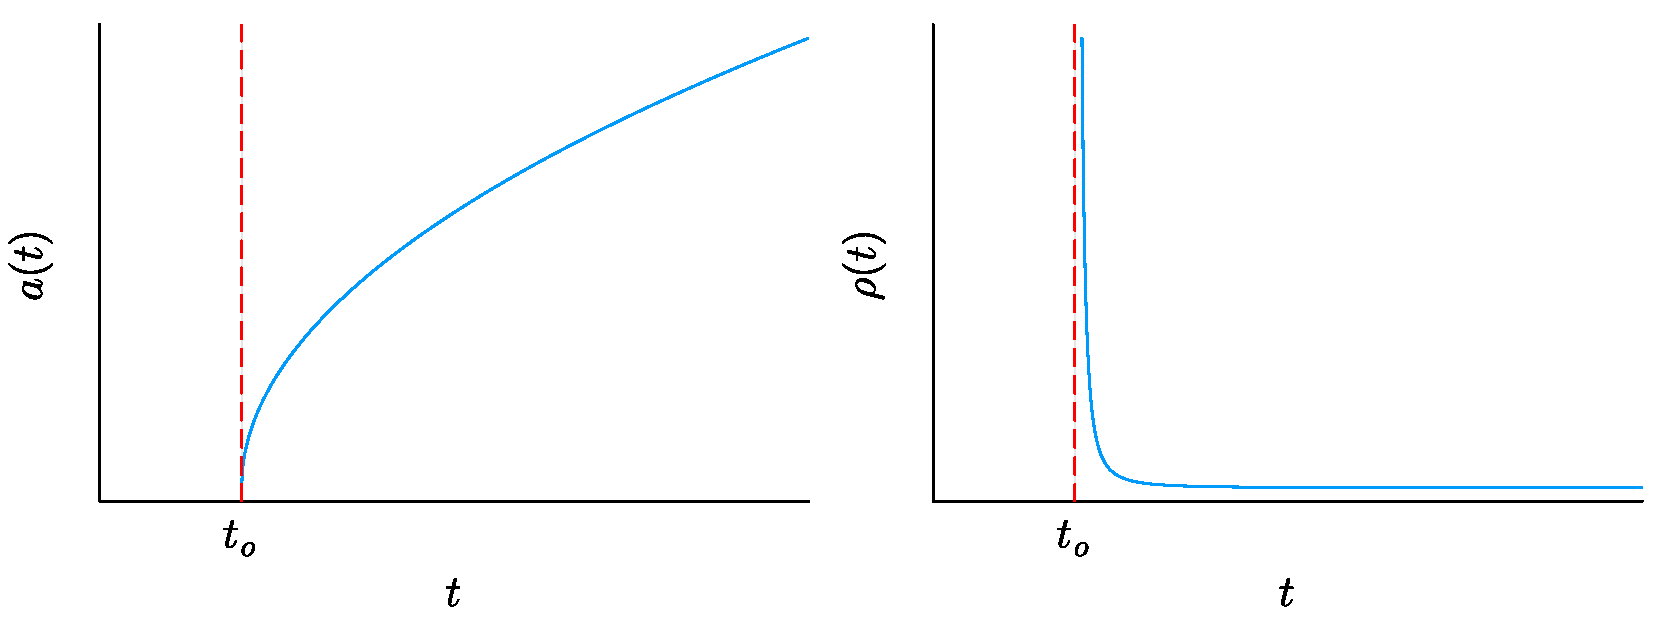
\includegraphics[scale=0.5]{pics/lec28_1.pdf}
    \caption{Plot of $a(t)$ and $\rho(t)$ with time in a radiation dominated Universe}
\end{figure}
Now, from the expression of $a(t)$ we can find the density profile,
$$\rho(t) = \rho\tund{0}\qty(\frac{a\tund{0}}{c\tund{0}\sqrt{t-t\tund{0}}})^4 \sim \frac{1}{(t-t\tund{0})^2}$$
This blows up as $t\to t\tund{0}$ and things kinda becomes \textit{unphysical}! This implies that, during the Big Bang, the energy density of the Universe was infinite. We suspect that GR might break down at $t\tund{0}$ since this predicts something unphysical. Perhaps a theory of \textit{quantisation of gravity}, if it occurs someday, may be able to rescue this apparent breakdown!\\[0.2cm]
\subsection{Pressureless matter}
We will now look at a simpler case of pressureless \textit{dust matter}, that is, $P=0$. Using this in the Friedmann equation we obtain,
$$\dot{\rho} = -3 \qty(\frac{\dot{a}}{a}) \implies \frac{\dd \rho}{\rho} = -3 \frac{\dd a}{a} \implies \boxed{\rho = \rho\tund{0}\qty(\frac{a\tund{0}}{a})^3}$$ 
Now using this in the Friedmann equation we obtain 
\begin{align*}
    \qty(\frac{\dot{a}}{a})^2 = \frac{8\pi G\rho\tund{0}}{3} \qty(\frac{a\tund{0}}{a})^3 \implies \dot{a} = \sqrt{\frac{8\pi G \rho\tund{0}a\tund{0}^3}{3}}\frac{1}{\sqrt{a}} \implies  a(t) \sim (t-t\tund{0})^{\sfrac{2}{3}}
\end{align*}
And we also look at the energy density 
$$\rho(t) = \rho\tund{0}\qty(\frac{a\tund{0}}{a})^3 \sim \frac{1}{(t-t\tund{0})^2}$$
We see that the energy density profile remains same for the pressureless matter case also, that is, it has a singularity at $t=t\tund{0}$. 
\begin{figure}[H]
    \centering
    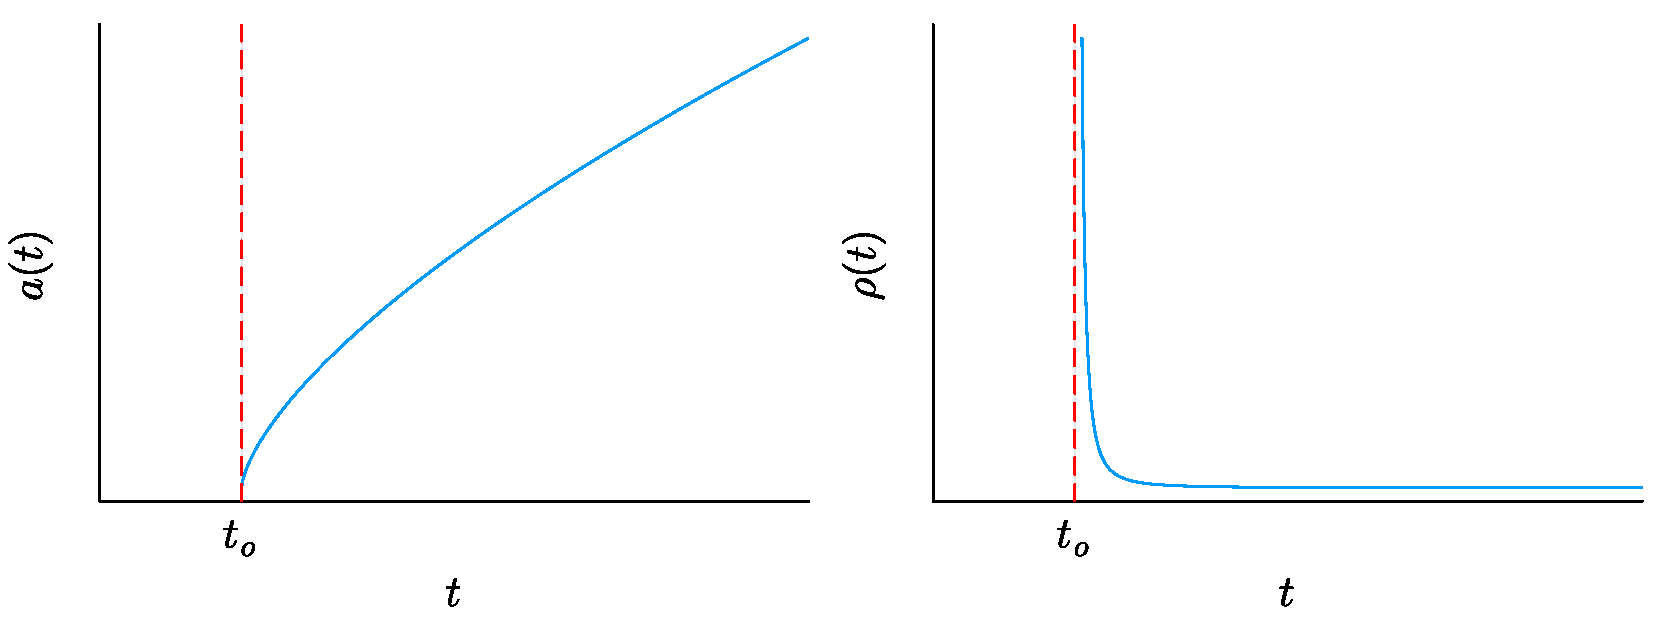
\includegraphics[scale=0.4]{pics/lec28_2.pdf}
    \caption{Plot of $a(t)$ and $\rho(t)$ with time for a pressureless dust matter}
\end{figure}